% !TeX root = ../main.tex

\chapter{Verwandte Arbeiten}\label{chapter:background}
	
	%In this chapter, \dots

	%\section{Math} \label{sec:full_grids}
	
		%Math:
		%\begin{align}
			%\Phi(x) = \max(1 - \abs{x}, 0)
		%\end{align}
		
	 %\subsection{Example Figure} \label{sec:back_nodal_hierarchical_basis}
		
		%\begin{figure}[htbp]
			%\centering
			%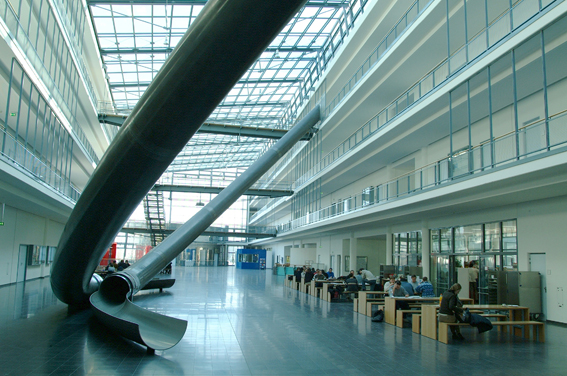
\includegraphics[width=0.5\textwidth]{figures/tum.jpg}
			%\caption{Example picture that was taken from an external source \takenFrom{asc_notes}.}
			%\label{fig:nodalBasis}
		%\end{figure}
		
		%References on figures work like this: blblablabla (see \refFigure{fig:nodalBasis}). If you used external knowledge for a paragraph, use the cite command at the very end of a sentence but right before the full stop \cite{ba_molzer}.
		
		%If you use an $l$ for math symbols, use $\ell$ instead for better readability.
		
	Vor dem Behandeln eines Problems ist es wichtig sich ebenso darüber zu informieren, was in diesem Bereich bereits in anderen Arbeiten behandelt wurde und welche Ergebnisse dabei erzielt wurden. Für diese Arbeit sind beispielsweise die Forschungen im Bereich der Platzierung von Benutzeroberflächen in 2D- und 3D-Anwendungen relevant, ebenso wie das Themenfeld der Priorisierung von anzuzeigenden Informationen.
	Während Forschungen im Bereich der Positionierung und des Designs von Nutzeroberflächen in Desktop-Anwendungen bereits auf jahrelange Erfahrung zurückblicken können, steht man dort bei HMD-Anwendungen noch relativ am Anfang.
	Auch bei dem Thema plattformübergreifender Programme in der erweiterten Realität gibt es schon einige Ansätze, wie ein Projekt von der Organisation Mozilla und eine Reihe von VR- und AR-Spielen zeigt \cite{firefox}\cite{crossCB}.
	Bei näherer Betrachtung dieser Programme fällt jedoch auf, dass hierbei nicht das ganze Potential zur Anzeige von Informationen ausgeschöpft wurde. 
		
	\section{Priorisieren von Benutzeroberflächen}\label{chapter:prio}
		Das Umstrukturieren von Menüs ist nicht trivial, denn jede Veränderung in der Benutzeroberfläche kann das Nutzererlebnis drastisch verändern, falls der Nutzer dadurch irritiert wird. Dies ist sowohl in zweidimensionalen Programmen der Fall, wie auch in der virtuellen dreidimensionalen Welt.
		Mit diesem Nutzererlebnis setzt sich seit einigen Jahren der Bereich des UX Designs (User Experience Design) auseinander.
		Ein wichtiger Aspekt davon ist es, dem Nutzer sowohl nicht zu viel als auch nicht zu wenig Informationen auf einmal zu geben. Dies könnte sonst zu einer Überfordert führen, beziehungsweise durch mangelnde Daten die Nutzung erschweren.
		Es gibt für dieses Problem jedoch keine klare Lösung, da es sich dabei um ein subjektives Erlebnis handelt.
		Um aber das Risiko einer Verschlechterung des Nutzungserlebnisses gering zu halten, hilft es die vorhandenen Informationen zu priorisieren und abhängig davon zu entscheiden, wann und wie diese dem Nutzer angezeigt werden. Dazu verwendet man normalerweise Untermenüs, Tabs oder Ähnliches.\cite{UXNatoli}
		
		
		Dies lässt bereits eine klare Priorisierung erkennen.
		Ausgehend von der Darstellung eines Elements der Benutzeroberfläche in einem Desktop-Programm, kann dessen Wichtigkeit in vier grobe Kategorien einteilt werden.
		
		In die Kategorie mit der höchsten Priorität fallen jene Objekte, die immer angezeigt werden, egal wie das Programmfenster verformt wird. Notfalls wird dafür sogar die Skalierung eingeschränkt. Typische Beispiele für diese Kategorie sind die \term{Speichern}- und die \term{Programm Schließen}-Schaltflächen.
		
		Etwas weniger wichtige Informationen werden zwar auch immer versucht anzuzeigen, aber falls der Platz dafür nicht ausreichen sollte, werden sie etwa in ein temporäres Untermenü verschoben oder auf andere Weise minimiert. Sobald wieder genug Platz vorhanden ist, tauchen sie erneut an der gewohnten Stelle auf. Dazu zählen unter anderem Hilfsfunktionen, wie das \term{Einfügen} oder \term{Ausschneiden} in Texteditoren.
		
		Untermenüs beherbergen die nächst tiefere Kategorie. Deren Inhalt kann manuell angezeigt werden, aber ist sonst nie sichtbar. Es handelt sich meist um sekundäre Funktionen, die nur gelegentlich benötigt werden.
		
		Die unwichtigsten Elemente befinden sich in Menüs innerhalb von Untermenüs und sind somit nur durch mehrere Interaktionen auffindbar. Im Normalfall sind dieses Einstellungen, welche nur selten verwendet werden.
		%- Elemente immer angezeigt (typisch Speichern und Exit)
		%- Elemente können versteckt werden (Funktionen Einfügen/Ausschneiden)
		%- Elemente in Untermenü (dropdown)
		%- elemente in Unteruntermenüs (Funktionen, die selten verwendet werden z.B Einstellungen)
		
		Tabs erzeugen jedoch Ausnahmen bei dieser Einordnung. Sie stellen sozusagen verschiedene Kontexte dar, in welchen die Prioritäten anders verteilt sein können. So existieren möglicherweise in einem Kontext bestimmte Informationen nicht, aber in einem anderen werden sie durchgehend angezeigt. Aus diesem Grund wird zwischen kontextabhängigen und -unabhängigen Elementen unterschieden.
		
		%- UX
		%- Prioritätsgruppen
		%- Umsetzung in 2D
		
	\section{Positionierung in 2D-Anwendungen}
		Das verbreitetste Konzept bei der Erstellung von Nutzeroberflächen ist das WIMP-Konzept. Die Abkürzung steht für \term{Windows}, \term{Icons}, \term{Menus} und \term{Pointers}. 
		Damit deutet sie bereits darauf hin, wie man sich die Umsetzung dieses Konzepts vorstellen kann. Programme werden bei dieser nämlich als Fenster dargestellt. Diese können weitere Fenster enthalten oder auch Menüs, in welchen Inhalte angeordnet sind. Um Funktionen möglichst kompakt anzeigen zu können, werden diese teilweise in Form von einem Bild oder Zeichen, einem sogenannten \term{Icon} dargestellt.
		Als Anker zum Positionieren des Fensterinhalts dienen jeweils die Eckpunkte des Fensters. Die einzelnen Elemente werden in den Fenstern also immer relativ zu mindestens einer Ecke des jeweiligen Fensters platziert. Dadurch kann der Inhalt eines Programmfensters bei dessen Verschiebung oder Skalierung mitbeweget werden. Damit ein Objekt sich zudem mit dem enthaltenden Bildausschnitt vergrößert, verkleinert oder darin zentriert bleibt, muss es hingegen an zwei oder mehr Ecken gebunden werden. Dies wird in der \refFigure{fig:unity} aus der Spiel-Engine Unity am rechten und unteren Rand dargestellt.
		%Damit sich Programmfenster beliebig vergrößern lassen, auch unabhängig von den ursprünglichen Seitenlängenverhältnissen, ohne dass der Inhalt an einer Seite abrupt abgeschnitten wird, muss 
		%- Windows Icons Menus Pointers
		
		%- Menüs / Fenster
		%Menüs geben eine Auswahl von Funktionen in Form von ...
		%- Bildschirmränder
		
		
	\section{Positionierung in 3D-Anwendungen}\label{chapter:3dPos}
		
		In Programmen, die eine dreidimensionale virtuelle Welt anzeigen (im Folgenden \term{3D-Programm} genannt), wird eine spezielle Form der graphischen Benutzeroberfläche verwendet. Diese liegt nicht in einer zweidimensionalen Ebene vor der Kamera, sondern befindet sich im dreidimensionalen Raum. Dies ermöglicht auch nicht-planare Formen, was dieser Abwandlung den Namen \term{3D User Interface} gab.
		
		Diese dreidimensionalen Elemente werden in 3D-Programmen für Desktop-Geräte gewöhnlich an festen Orten angebracht und bewegt sich gegebenenfalls an einem Objekt der Umgebung mit. Dies wird auch als diegetische Benutzeroberfläche bezeichnet, da sie tatsächlich Teil der virtuellen Welt ist.
		
		In VR- und AR-Anwendungen steht teilweise zusätzlich die Option zur Verfügung, einen virtuellen Gegenstand oder eine Anzeige an den Handpositionen des Nutzers zu befestigen, oder ihn mit der Nutzeroberfläche auf andere Arten räumlich zu umgeben. Dies bietet dem Benutzer eine natürliche Art der Interaktion. Um etwas auszuwählen könnte er einfach auf das gewünschte Element zugehen und nach ihm die Hand ausstrecken. Denkbar ist eine solche Umsetzung unter anderem in Form eines Zylinders, wie in \refFigure{fig:cylinder_mapping} dargestellt.
		
		%- 3D Programm: UI in Welt platziert
		%- Üblich Hände und Kopf oder an statischen Objekten
		In dieser Arbeit wurden als Ankerpunkte für solche Elemente die beiden Handpositionen des Benutzers und die Kopfposition verwendet, da diese Stellen im Fall der Verwendung von Erfassungssystemen durch Controller, das HMD oder die reale Hand gegeben sind.
		
		\begin{figure}[htbp]
			\centering
			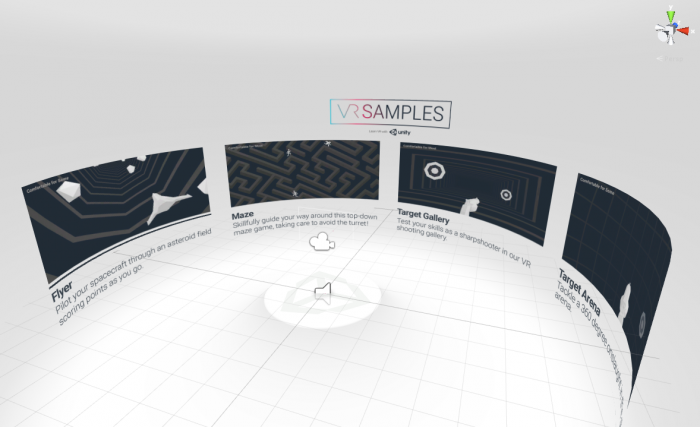
\includegraphics[width=0.75\textwidth]{figures/cylinder_mapping.png}
			\caption{Example picture that was taken from an external source \takenFrom{unityCurved}.}
			\label{fig:cylinder_mapping}
		\end{figure}